% Artigo final de Biometria (UTFPR). Template IEEE conference (IEEEtran).
% Se a professora definir SBC, o conteúdo das seções se mantém; trocar só o preâmbulo.
% Números: % Gerado por artigo/gerar_numeros.py. Não editar à mão.
\newcommand{\repourl}{\url{https://github.com/felipesilveirasouza/biometria-projeto-final}}
\newcommand{\eerCFP}{5{,}09}
\newcommand{\aucCFP}{0{,}9840}
\newcommand{\tarCFP}{89{,}80}
\newcommand{\ftaCFP}{1{,}56}
\newcommand{\fmrCFP}{5{,}06 $\pm$ 1{,}32}
\newcommand{\fnmrCFP}{5{,}06 $\pm$ 1{,}82}
\newcommand{\accCFP}{94{,}94 $\pm$ 1{,}34}
\newcommand{\eerLFW}{0{,}57}
\newcommand{\aucLFW}{0{,}9995}
\newcommand{\tarLFW}{99{,}60}
\newcommand{\ftaLFW}{0{,}01}
\newcommand{\fmrLFW}{0{,}60 $\pm$ 0{,}49}
\newcommand{\fnmrLFW}{0{,}63 $\pm$ 0{,}74}
\newcommand{\accLFW}{99{,}38 $\pm$ 0{,}39}
\newcommand{\eerFF}{1{,}00}
\newcommand{\aucFF}{0{,}9992}
\newcommand{\tarFF}{99{,}09}
\newcommand{\ftaFF}{0{,}19}
\newcommand{\fmrFF}{1{,}00 $\pm$ 0{,}61}
\newcommand{\fnmrFF}{1{,}03 $\pm$ 0{,}70}
\newcommand{\accFF}{98{,}99 $\pm$ 0{,}57}
\newcommand{\eerAlnCFP}{6{,}16}
\newcommand{\aucAlnCFP}{0{,}9825}
\newcommand{\tarAlnCFP}{85{,}97}
\newcommand{\ftaAlnCFP}{1{,}56}
\newcommand{\fmrAlnCFP}{6{,}20 $\pm$ 1{,}81}
\newcommand{\fnmrAlnCFP}{6{,}14 $\pm$ 2{,}33}
\newcommand{\accAlnCFP}{93{,}83 $\pm$ 1{,}85}
\newcommand{\eerAlnLFW}{0{,}88}
\newcommand{\aucAlnLFW}{0{,}9994}
\newcommand{\tarAlnLFW}{99{,}23}
\newcommand{\ftaAlnLFW}{0{,}01}
\newcommand{\fmrAlnLFW}{0{,}93 $\pm$ 0{,}41}
\newcommand{\fnmrAlnLFW}{0{,}90 $\pm$ 0{,}90}
\newcommand{\accAlnLFW}{99{,}08 $\pm$ 0{,}49}
\newcommand{\thrCFP}{0{,}256}
\newcommand{\thrLFW}{0{,}410}
\newcommand{\thrFF}{0{,}376}
\newcommand{\fmrCross}{6{,}73}
\newcommand{\fnmrCross}{0{,}17}
\newcommand{\accCross}{96{,}55}
\newcommand{\alignCFP}{68{,}4\%}
\newcommand{\alignLFW}{99{,}7\%}
\newcommand{\ablWinsCFP}{7}
\newcommand{\ablTiesCFP}{1}
\newcommand{\ablDiffCFP}{1{,}11}
\newcommand{\ablPCFP}{0{,}020}
\newcommand{\ablWinsLFW}{6}
\newcommand{\ablTiesLFW}{1}
\newcommand{\ablDiffLFW}{0{,}30}
\newcommand{\ablPLFW}{0{,}074}
\newcommand{\nFmCross}{202}
\newcommand{\nFmCrossLFW}{17}
\newcommand{\muGenCFP}{0{,}58}
\newcommand{\muImpCFP}{0{,}01}
\newcommand{\muGenLFW}{0{,}78}
\newcommand{\muImpLFW}{0{,}02}
\newcommand{\muGenFF}{0{,}75}
\newcommand{\muImpFF}{0{,}01}
\newcommand{\ftaFrontal}{0{,}18}
\newcommand{\ftaPerfil}{4{,}33}
\newcommand{\landmarksPerfil}{21{,}3\%}
\newcommand{\landmarksFrontal}{91{,}9\%}
\newcommand{\eerBlurOrig}{5{,}09}
\newcommand{\fnmrBlurOrig}{5{,}06}
\newcommand{\fmrBlurOrig}{5{,}06}
\newcommand{\ftaBlurOrig}{--}
\newcommand{\eerBlurBaixa}{6{,}16}
\newcommand{\fnmrBlurBaixa}{6{,}80}
\newcommand{\fmrBlurBaixa}{4{,}94}
\newcommand{\ftaBlurBaixa}{4{,}64}
\newcommand{\eerBlurMedia}{11{,}17}
\newcommand{\fnmrBlurMedia}{16{,}46}
\newcommand{\fmrBlurMedia}{5{,}11}
\newcommand{\ftaBlurMedia}{6{,}94}
\newcommand{\eerBlurAlta}{21{,}70}
\newcommand{\fnmrBlurAlta}{37{,}37}
\newcommand{\fmrBlurAlta}{4{,}20}
\newcommand{\ftaBlurAlta}{13{,}92}
\newcommand{\eerOclOrig}{5{,}09}
\newcommand{\fnmrOclOrig}{5{,}06}
\newcommand{\fmrOclOrig}{5{,}06}
\newcommand{\ftaOclOrig}{--}
\newcommand{\eerOclBaixa}{5{,}36}
\newcommand{\fnmrOclBaixa}{5{,}60}
\newcommand{\fmrOclBaixa}{5{,}17}
\newcommand{\ftaOclBaixa}{4{,}33}
\newcommand{\eerOclMedia}{7{,}04}
\newcommand{\fnmrOclMedia}{9{,}00}
\newcommand{\fmrOclMedia}{4{,}51}
\newcommand{\ftaOclMedia}{4{,}33}
\newcommand{\eerOclAlta}{10{,}91}
\newcommand{\fnmrOclAlta}{17{,}91}
\newcommand{\fmrOclAlta}{4{,}14}
\newcommand{\ftaOclAlta}{4{,}33}
\newcommand{\paramsM}{23{,}48}
\newcommand{\pesoMB}{89{,}9}
\newcommand{\msBatchOne}{22{,}3}
\newcommand{\msBatch}{3{,}66}
\newcommand{\cpu}{AMD Ryzen 7 1700 Eight-Core Processor}
\newcommand{\gpu}{NVIDIA GeForce GTX 1050 Ti}
\newcommand{\torchv}{2.2.2\texttt{+}cu121}
\newcommand{\pythonv}{3.12.16}
 é gerado por `python artigo/gerar_numeros.py` a partir de results/.
\documentclass[conference,a4paper]{IEEEtran}
\usepackage[utf8]{inputenc}
\usepackage[T1]{fontenc}
\usepackage[brazilian]{babel}
\usepackage{graphicx}
\usepackage{booktabs}
\usepackage{amsmath,amssymb}
\usepackage{siunitx}
\usepackage{xcolor}
\usepackage[hidelinks]{hyperref}
\usepackage{cite}
\sisetup{output-decimal-marker={,}}
\graphicspath{{../results/}{figuras/}}
\newcommand{\todo}[1]{\textcolor{red}{[TODO: #1]}}
% Gerado por artigo/gerar_numeros.py. Não editar à mão.
\newcommand{\repourl}{\url{https://github.com/felipesilveirasouza/biometria-projeto-final}}
\newcommand{\eerCFP}{5{,}09}
\newcommand{\aucCFP}{0{,}9840}
\newcommand{\tarCFP}{89{,}80}
\newcommand{\ftaCFP}{1{,}56}
\newcommand{\fmrCFP}{5{,}06 $\pm$ 1{,}32}
\newcommand{\fnmrCFP}{5{,}06 $\pm$ 1{,}82}
\newcommand{\accCFP}{94{,}94 $\pm$ 1{,}34}
\newcommand{\eerLFW}{0{,}57}
\newcommand{\aucLFW}{0{,}9995}
\newcommand{\tarLFW}{99{,}60}
\newcommand{\ftaLFW}{0{,}01}
\newcommand{\fmrLFW}{0{,}60 $\pm$ 0{,}49}
\newcommand{\fnmrLFW}{0{,}63 $\pm$ 0{,}74}
\newcommand{\accLFW}{99{,}38 $\pm$ 0{,}39}
\newcommand{\eerFF}{1{,}00}
\newcommand{\aucFF}{0{,}9992}
\newcommand{\tarFF}{99{,}09}
\newcommand{\ftaFF}{0{,}19}
\newcommand{\fmrFF}{1{,}00 $\pm$ 0{,}61}
\newcommand{\fnmrFF}{1{,}03 $\pm$ 0{,}70}
\newcommand{\accFF}{98{,}99 $\pm$ 0{,}57}
\newcommand{\eerAlnCFP}{6{,}16}
\newcommand{\aucAlnCFP}{0{,}9825}
\newcommand{\tarAlnCFP}{85{,}97}
\newcommand{\ftaAlnCFP}{1{,}56}
\newcommand{\fmrAlnCFP}{6{,}20 $\pm$ 1{,}81}
\newcommand{\fnmrAlnCFP}{6{,}14 $\pm$ 2{,}33}
\newcommand{\accAlnCFP}{93{,}83 $\pm$ 1{,}85}
\newcommand{\eerAlnLFW}{0{,}88}
\newcommand{\aucAlnLFW}{0{,}9994}
\newcommand{\tarAlnLFW}{99{,}23}
\newcommand{\ftaAlnLFW}{0{,}01}
\newcommand{\fmrAlnLFW}{0{,}93 $\pm$ 0{,}41}
\newcommand{\fnmrAlnLFW}{0{,}90 $\pm$ 0{,}90}
\newcommand{\accAlnLFW}{99{,}08 $\pm$ 0{,}49}
\newcommand{\thrCFP}{0{,}256}
\newcommand{\thrLFW}{0{,}410}
\newcommand{\thrFF}{0{,}376}
\newcommand{\fmrCross}{6{,}73}
\newcommand{\fnmrCross}{0{,}17}
\newcommand{\accCross}{96{,}55}
\newcommand{\alignCFP}{68{,}4\%}
\newcommand{\alignLFW}{99{,}7\%}
\newcommand{\ablWinsCFP}{7}
\newcommand{\ablTiesCFP}{1}
\newcommand{\ablDiffCFP}{1{,}11}
\newcommand{\ablPCFP}{0{,}020}
\newcommand{\ablWinsLFW}{6}
\newcommand{\ablTiesLFW}{1}
\newcommand{\ablDiffLFW}{0{,}30}
\newcommand{\ablPLFW}{0{,}074}
\newcommand{\nFmCross}{202}
\newcommand{\nFmCrossLFW}{17}
\newcommand{\muGenCFP}{0{,}58}
\newcommand{\muImpCFP}{0{,}01}
\newcommand{\muGenLFW}{0{,}78}
\newcommand{\muImpLFW}{0{,}02}
\newcommand{\muGenFF}{0{,}75}
\newcommand{\muImpFF}{0{,}01}
\newcommand{\ftaFrontal}{0{,}18}
\newcommand{\ftaPerfil}{4{,}33}
\newcommand{\landmarksPerfil}{21{,}3\%}
\newcommand{\landmarksFrontal}{91{,}9\%}
\newcommand{\eerBlurOrig}{5{,}09}
\newcommand{\fnmrBlurOrig}{5{,}06}
\newcommand{\fmrBlurOrig}{5{,}06}
\newcommand{\ftaBlurOrig}{--}
\newcommand{\eerBlurBaixa}{6{,}16}
\newcommand{\fnmrBlurBaixa}{6{,}80}
\newcommand{\fmrBlurBaixa}{4{,}94}
\newcommand{\ftaBlurBaixa}{4{,}64}
\newcommand{\eerBlurMedia}{11{,}17}
\newcommand{\fnmrBlurMedia}{16{,}46}
\newcommand{\fmrBlurMedia}{5{,}11}
\newcommand{\ftaBlurMedia}{6{,}94}
\newcommand{\eerBlurAlta}{21{,}70}
\newcommand{\fnmrBlurAlta}{37{,}37}
\newcommand{\fmrBlurAlta}{4{,}20}
\newcommand{\ftaBlurAlta}{13{,}92}
\newcommand{\eerOclOrig}{5{,}09}
\newcommand{\fnmrOclOrig}{5{,}06}
\newcommand{\fmrOclOrig}{5{,}06}
\newcommand{\ftaOclOrig}{--}
\newcommand{\eerOclBaixa}{5{,}36}
\newcommand{\fnmrOclBaixa}{5{,}60}
\newcommand{\fmrOclBaixa}{5{,}17}
\newcommand{\ftaOclBaixa}{4{,}33}
\newcommand{\eerOclMedia}{7{,}04}
\newcommand{\fnmrOclMedia}{9{,}00}
\newcommand{\fmrOclMedia}{4{,}51}
\newcommand{\ftaOclMedia}{4{,}33}
\newcommand{\eerOclAlta}{10{,}91}
\newcommand{\fnmrOclAlta}{17{,}91}
\newcommand{\fmrOclAlta}{4{,}14}
\newcommand{\ftaOclAlta}{4{,}33}
\newcommand{\paramsM}{23{,}48}
\newcommand{\pesoMB}{89{,}9}
\newcommand{\msBatchOne}{22{,}3}
\newcommand{\msBatch}{3{,}66}
\newcommand{\cpu}{AMD Ryzen 7 1700 Eight-Core Processor}
\newcommand{\gpu}{NVIDIA GeForce GTX 1050 Ti}
\newcommand{\torchv}{2.2.2\texttt{+}cu121}
\newcommand{\pythonv}{3.12.16}


\begin{document}

\title{Verificação Facial Frontal $\times$ Perfil com Inception-ResNet-v1:\\
Avaliação em CFP-FP, Generalização para LFW e Robustez}

\author{\IEEEauthorblockN{Felipe Silveira}
\IEEEauthorblockA{Biometria --- Universidade Tecnológica Federal do Paraná (UTFPR)\\
Câmpus Ponta Grossa}}

\maketitle

\begin{abstract}
\todo{escrever por último (150--200 palavras): problema (verificação 1:1 frontal
$\times$ perfil), método (Inception-ResNet-v1 pré-treinada no VGGFace2, congelada,
cosseno), protocolo (10 folds oficiais, threshold na validação), principais números
(EER CFP-FP \eerCFP, LFW \eerLFW, cross-dataset), achado principal (alinhamento /
perfil / robustez).}
\end{abstract}

\begin{IEEEkeywords}
biometria, verificação facial, FaceNet, CFP-FP, LFW, robustez
\end{IEEEkeywords}

% =====================================================================
\section{Introdução}
% problema, modalidade, motivação, objetivo e contribuição
Um sistema de verificação biométrica responde a uma pergunta 1:1: a amostra
apresentada pertence à identidade declarada? Para isso, ele extrai de cada amostra um
template, compara os dois templates por uma medida de similaridade e aceita o par
quando o score supera um limiar de decisão~\cite{jain2004introduction}. Os erros
possíveis são aceitar um impostor (\emph{false match}) e rejeitar um usuário genuíno
(\emph{false non-match}), cujas taxas, FMR e FNMR, dependem do limiar
escolhido~\cite{iso19795}.

A face é uma das modalidades mais usadas por ser adquirida sem contato, à distância e
com câmeras comuns. Com redes convolucionais profundas treinadas em milhões de
imagens, o reconhecimento facial passou a ter acurácia acima de 99\% em fotos quase
frontais~\cite{wang2021deep}. O desempenho, porém, cai em condições menos
controladas: variação de pose, iluminação, oclusão e baixa resolução continuam sendo
as principais fontes de erro. A pose é um caso especialmente difícil, porque uma foto
de perfil esconde metade do rosto e muda a geometria de todos os traços visíveis. A
base CFP~\cite{sengupta2016frontal} foi criada para isolar esse fator: seu protocolo
FP compara uma foto frontal com uma de perfil da mesma pessoa ou de pessoas
diferentes, e o desempenho de humanos e de algoritmos é menor nele do que na
comparação entre duas frontais.

\textbf{Objetivo.} Este trabalho avalia um sistema de verificação facial baseado em
embeddings de uma CNN pré-treinada, a Inception-ResNet-v1 do
FaceNet~\cite{schroff2015facenet,szegedy2017inception}, usada sem
\emph{fine-tuning}, no cenário frontal $\times$ perfil do CFP-FP. Além disso, mede
quanto o sistema generaliza para outra base (LFW), com o limiar congelado, e quanto
resiste a degradações da imagem. Todo o protocolo segue as divisões oficiais das
bases, e o limiar é escolhido apenas na validação.

\textbf{Contribuições.}
(i) avaliação reprodutível no CFP-FP (EER de \eerCFP\%) e no LFW (EER de
\eerLFW\%) com os 10 folds oficiais;
(ii) experimento cross-dataset que quantifica o custo de usar no LFW o limiar
calibrado no CFP-FP;
(iii) análise de robustez a desfoque e oclusão em quatro níveis;
(iv) ablação do pré-processamento, mostrando que alinhar a face pelo template de
5 pontos do ArcFace \emph{piora} o desempenho de uma rede pré-treinada com recortes
pela bbox;
(v) análise qualitativa de falsos matches e falsos non-matches. O código e os
resultados estão disponíveis em \repourl.

% =====================================================================
\section{Trabalhos relacionados}
% métodos da literatura, CNNs e resultados de referência
\textbf{Da engenharia de características às CNNs.} Os primeiros sistemas de
reconhecimento facial representavam a face por projeções lineares, como as
Eigenfaces~\cite{turk1991eigenfaces}, ou por descritores de textura locais, como os
histogramas de LBP~\cite{ahonen2006face}. Essas representações são sensíveis a pose e
iluminação. O DeepFace~\cite{taigman2014deepface} mostrou que uma CNN treinada em
milhões de faces, combinada com alinhamento 3D, chegava a 97,35\% de acurácia no LFW,
perto do desempenho humano. Em seguida, o VGG-Face~\cite{parkhi2015deep} mostrou que
uma arquitetura convolucional profunda e uma base de treino grande, coletada
automaticamente, bastavam para resultados competitivos.

\textbf{Aprendizado de embeddings.} O FaceNet~\cite{schroff2015facenet} passou a
treinar a rede para produzir diretamente um embedding em que a distância euclidiana
reflete a similaridade entre faces, com a \emph{triplet loss}, e obteve 99,63\% no
LFW. Trabalhos seguintes trocaram a triplet loss por variantes da softmax com margem
angular, mais estáveis de treinar: SphereFace~\cite{liu2017sphereface} (99,42\% no
LFW), CosFace~\cite{wang2018cosface} (99,73\%) e ArcFace~\cite{deng2019arcface}, que
se tornou a referência mais usada. Nesses métodos a comparação é feita pela
similaridade de cosseno entre embeddings normalizados, o mesmo esquema de matching
adotado aqui.

\textbf{Pose.} Sengupta et al.~\cite{sengupta2016frontal} mostraram, ao propor o CFP,
que tanto humanos quanto os algoritmos da época perdiam desempenho da comparação
frontal-frontal para a frontal-perfil. Para reduzir essa diferença, foram propostas
abordagens que geram uma vista frontal sintética ou aprendem representações
invariantes à pose, como o DR-GAN~\cite{tran2017disentangled}, e abordagens que
corrigem o embedding de perfis para aproximá-lo do de frontais, como o
DREAM~\cite{cao2018pose}. Os métodos atuais de margem angular, treinados em bases com
grande variação de pose como o VGGFace2~\cite{cao2018vggface2}, reduzem essa
diferença sem módulos específicos para pose.

\textbf{Arquitetura usada.} A Inception-ResNet~\cite{szegedy2017inception} combina os
módulos Inception, que processam a entrada em paralelo com filtros de tamanhos
diferentes, com as conexões residuais da ResNet~\cite{he2016deep}, que facilitam o
treino de redes profundas. A versão v1 é a base da implementação aberta do
FaceNet~\cite{sandberg_facenet}; o modelo pré-treinado no VGGFace2 com softmax de
identidade reporta 99,65\% $\pm$ 0,25\% de acurácia no LFW. Neste trabalho, ela é
usada como extratora de características congelada, sem nenhum treino nas bases de
avaliação.

% =====================================================================
\section{Bases de dados}
% indivíduos, amostras, aquisição, protocolo e exemplos
\textbf{CFP-FP (base principal).} O \emph{Celebrities in Frontal-Profile}~\cite{sengupta2016frontal}
contém 500 identidades, cada uma com 10 imagens frontais e 4 de perfil coletadas na
internet (\num{7000} imagens). O protocolo FP compara uma imagem frontal com uma de
perfil e é dividido em 10 folds de 350 pares genuínos e 350 impostores
(\num{7000} pares, \num{5901} imagens distintas usadas).

\textbf{LFW (segunda base).} O \emph{Labeled Faces in the Wild}~\cite{huang2007labeled}
tem \num{13233} imagens de \num{5749} pessoas, também coletadas da internet, com pose
predominantemente quase frontal. Usa-se a View~2: 10 folds de 300 pares genuínos e 300
impostores (\num{6000} pares, \num{7701} imagens, \num{4281} identidades).

Nas duas bases os folds oficiais são disjuntos por identidade, o que foi verificado
automaticamente (\texttt{make\_protocols.py}). A Fig.~\ref{fig:pipeline} mostra exemplos.

% =====================================================================
\section{Metodologia}
% pipeline, pré-processamento, CNN, treinamento/fine-tuning, embedding e matching
\subsection{Pipeline}
Imagem bruta $\rightarrow$ controle de qualidade $\rightarrow$ detecção (MTCNN~\cite{zhang2016joint},
bbox e 5 landmarks) $\rightarrow$ seleção do rosto $\rightarrow$ recorte pela bbox, $160\times160$
$\rightarrow$ normalização $(x-127{,}5)/128$ $\rightarrow$ CNN $\rightarrow$ embedding
512-D normalizado em L2 $\rightarrow$ cosseno $\rightarrow$ decisão por threshold.

\begin{figure*}[t]
\centering
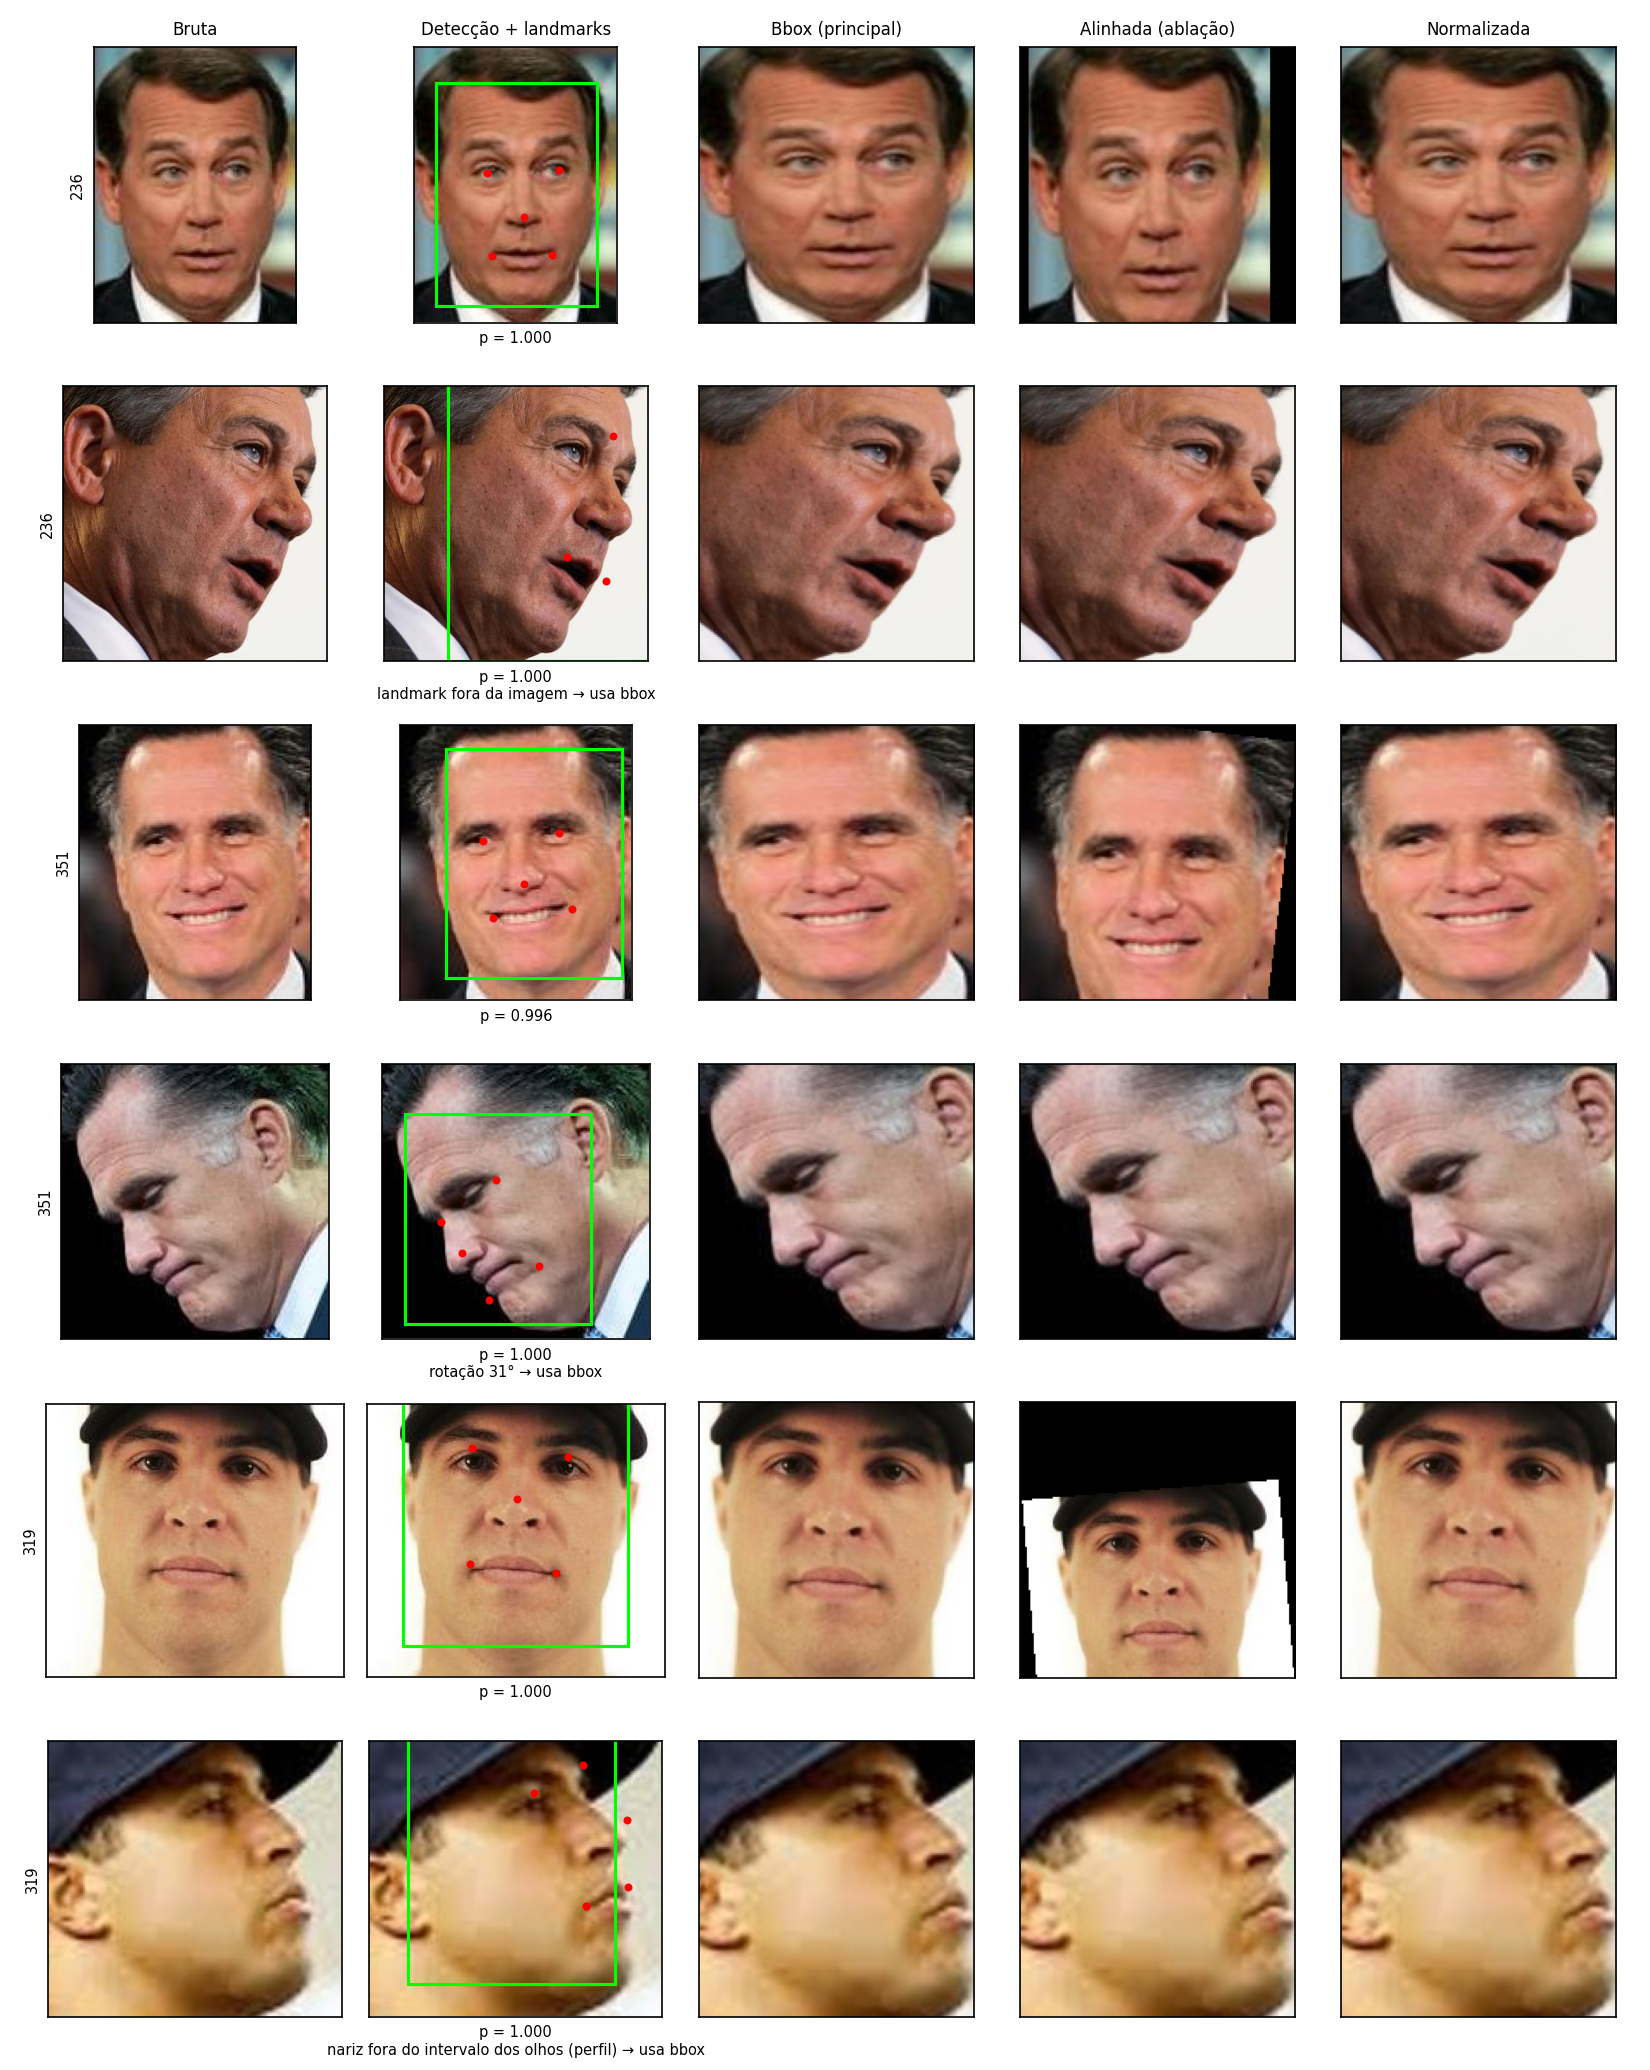
\includegraphics[width=\textwidth]{pipeline_cfp_fp.png}
\caption{Etapas do pré-processamento em pares genuínos do CFP-FP: imagem bruta,
detecção com landmarks, recorte pela bbox (principal), recorte alinhado por
landmarks (ablação) e entrada normalizada.
\todo{trocar/combinar com pipeline\_lfw.png se couber.}}
\label{fig:pipeline}
\end{figure*}

\subsection{Controle de qualidade e falha de aquisição}
Uma amostra é considerada falha de aquisição (FTA) se a imagem não abre ou se a MTCNN
não encontra rosto com probabilidade $\geq 0{,}90$. Nesse caso usa-se um recorte
central (política \emph{fallback}) e a falha é contabilizada.

\subsection{Seleção do rosto e recorte}
Quando a MTCNN detecta mais de um rosto, escolhe-se o de maior área penalizada pela
distância ao centro da imagem (o sujeito rotulado está centralizado nas duas bases),
critério usado pelo FaceNet original~\cite{sandberg_facenet}. Escolher apenas o maior
rosto seleciona pessoas ao fundo em parte das imagens do LFW; corrigir isso elevou a
acurácia no LFW de \todo{94,7\%} para \accLFW\%. O recorte é feito pela bbox com
margem de 20~px e redimensionado para $160\times160$, como no pré-treino do
modelo~\cite{sandberg_facenet}.

\textbf{Variante de ablação: alinhamento por landmarks.} Os 5 landmarks são levados ao
template de 5 pontos do ArcFace~\cite{deng2019arcface} por uma similaridade estimada
por mínimos quadrados~\cite{umeyama1991least}. Como o template é frontal, landmarks de
perfil frequentemente caem fora do rosto; aplica-se então uma verificação de
plausibilidade (landmarks dentro da imagem e da bbox, nariz entre os olhos, rotação
$\leq 30^\circ$) e, se falhar, usa-se a bbox. Foram alinhadas por landmarks
\alignCFP{} das imagens do CFP-FP e \alignLFW{} do LFW.

\subsection{CNN e embedding}
Inception-ResNet-v1~\cite{szegedy2017inception} com pesos da implementação
facenet-pytorch~\cite{esler_facenet_pytorch}, convertidos do modelo
\texttt{20180402-114759}~\cite{sandberg_facenet}, pré-treinado no
VGGFace2~\cite{cao2018vggface2} com perda softmax de identidade. A camada de
classificação é removida e todas as camadas permanecem congeladas (sem fine-tuning):
\paramsM{}M parâmetros, \pesoMB{}~MB, embedding de 512 dimensões.

\subsection{Matching e decisão}
O score é a similaridade de cosseno entre embeddings L2-normalizados. O par é aceito
como genuíno se o score for maior ou igual ao threshold $\tau$, escolhido no ponto de
EER do conjunto de validação.

% =====================================================================
\section{Protocolo experimental}
% divisões, pares, seeds, hardware, threshold, cross-dataset e robustez
\textbf{Divisões.} Em cada base, para cada fold $k$, $\tau$ é escolhido nos outros 9
folds (validação) e aplicado ao fold $k$ (teste). FMR, FNMR e acurácia são reportados como
média $\pm$ desvio-padrão dos 10 folds. EER, AUC e TAR@FAR=1\% independem de $\tau$ e
usam todos os pares. Como não há treino, não há conjunto de treino nem repetição com
seeds; a seed 42 fixa as posições das oclusões.

\textbf{Cross-dataset (C).} O threshold global do CFP-FP ($\tau=\thrCFP$) é congelado e
aplicado ao LFW sem nenhum ajuste.

\textbf{Robustez (D).} No CFP-FP, a segunda imagem de cada par é degradada e a primeira
fica limpa. Desfoque gaussiano com $\sigma\in\{0; 1{,}5; 3; 5\}$ aplicado à imagem bruta
(antes da detecção) e oclusão por bloco cinza com lado de $\{0; 15; 30; 45\}\%$ do
recorte, em posição aleatória determinística. Os thresholds são os do experimento limpo.

\textbf{Ablação.} Recorte pela bbox (principal) versus alinhamento por 5 landmarks, nas duas bases.

\textbf{Hardware.} \cpu, GPU \gpu{} (4~GB), PyTorch \torchv, Python \pythonv.

% =====================================================================
\section{Resultados}
% EER, FMR, FNMR, ROC/AUC, distribuições, eficiência e demais métricas
\begin{table}[t]
\centering
\caption{Resultados de verificação (FMR, FNMR e acurácia: média $\pm$ dp nos 10 folds).}
\label{tab:resultados}
\resizebox{\columnwidth}{!}{%
\begin{tabular}{lcccccc}
\toprule
Experimento & EER (\%) & AUC & FMR (\%) & FNMR (\%) & TAR@1\% & FTA (\%)\\
\midrule
A: CFP-FP & \eerCFP & \aucCFP & \fmrCFP & \fnmrCFP & \tarCFP & \ftaCFP\\
B: LFW & \eerLFW & \aucLFW & \fmrLFW & \fnmrLFW & \tarLFW & \ftaLFW\\
C: CFP-FP$\rightarrow$LFW & \eerLFW & \aucLFW & \fmrCross & \fnmrCross & \tarLFW & \ftaLFW\\
\midrule
Abl.: CFP-FP alinhado & \eerAlnCFP & \aucAlnCFP & \fmrAlnCFP & \fnmrAlnCFP & \tarAlnCFP & \ftaAlnCFP\\
Abl.: LFW alinhado & \eerAlnLFW & \aucAlnLFW & \fmrAlnLFW & \fnmrAlnLFW & \tarAlnLFW & \ftaAlnLFW\\
\bottomrule
\end{tabular}}
\end{table}

\begin{figure}[t]
\centering
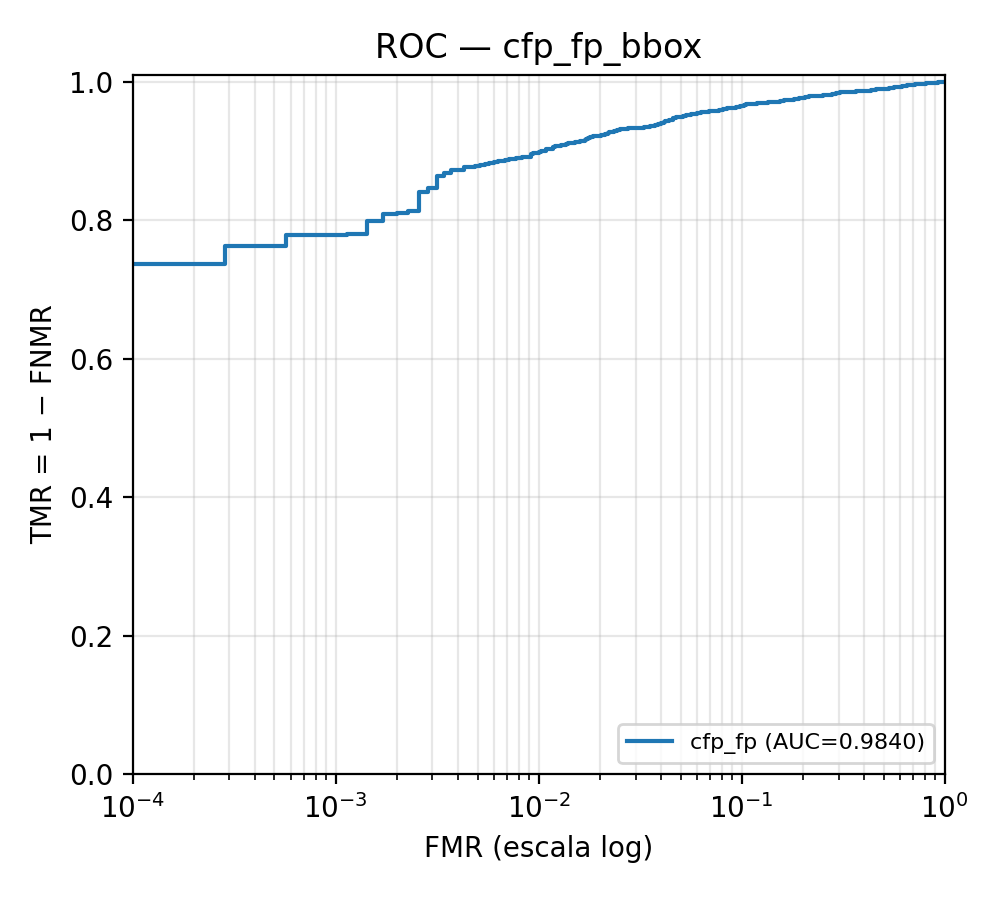
\includegraphics[width=\columnwidth]{cfp_fp_bbox/roc.png}
\caption{Curva ROC no CFP-FP. \todo{sobrepor LFW?}}
\label{fig:roc}
\end{figure}

\begin{figure}[t]
\centering
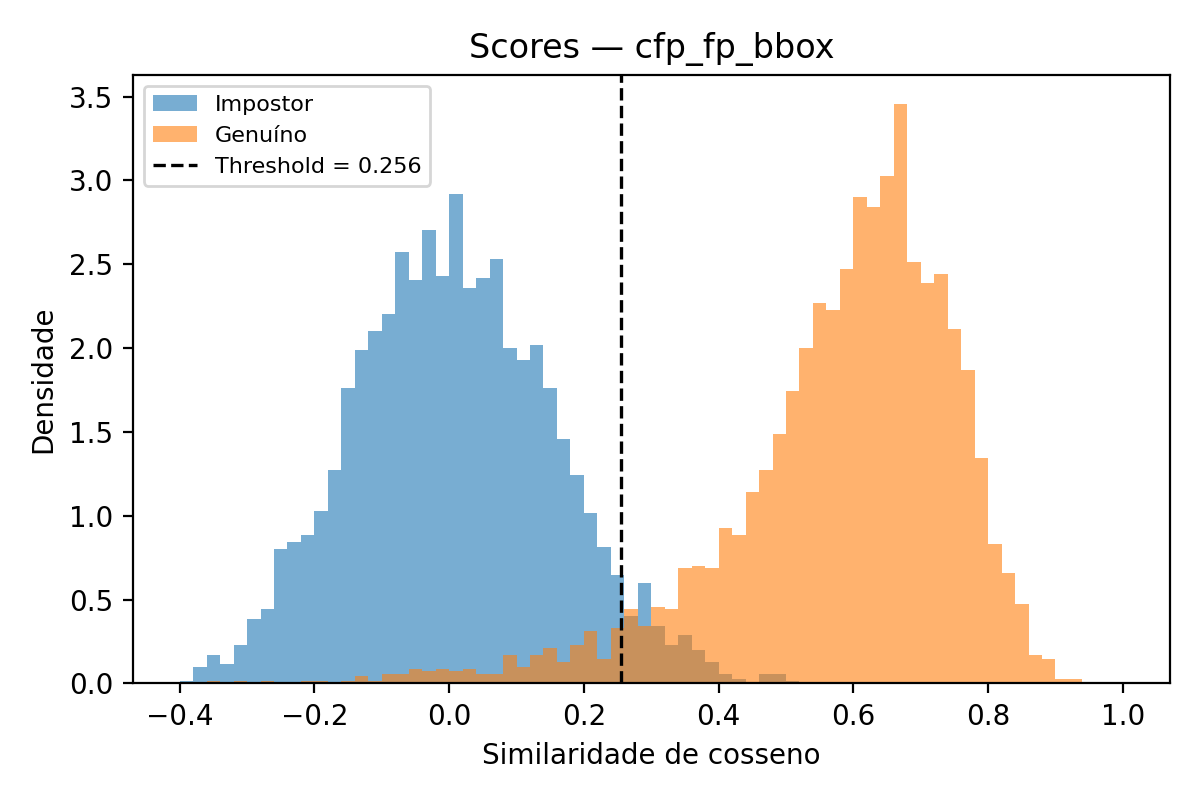
\includegraphics[width=\columnwidth]{cfp_fp_bbox/distributions.png}
\caption{Distribuição dos scores genuínos e impostores no CFP-FP, com o threshold.}
\label{fig:dist}
\end{figure}

\todo{Comentar Tab.~\ref{tab:resultados}, Figs.~\ref{fig:roc} e~\ref{fig:dist}:
separação das distribuições, sobreposição, onde ficam os erros.}

\textbf{Eficiência.} \msBatchOne~ms por imagem com batch 1 e \msBatch~ms com batch 64
na GPU (só a CNN; a MTCNN não está incluída).

% =====================================================================
\section{Análise e discussão}
% erros, cross-dataset, robustez, comparação, limitações
\subsection{Cross-dataset}
\todo{O threshold do CFP-FP (\thrCFP) é menor que o ótimo do LFW (\thrLFW): mais
impostores aceitos (FMR \fmrCross\%) e menos genuínos rejeitados (FNMR \fnmrCross\%).}

\subsection{Robustez}
\begin{figure}[t]
\centering
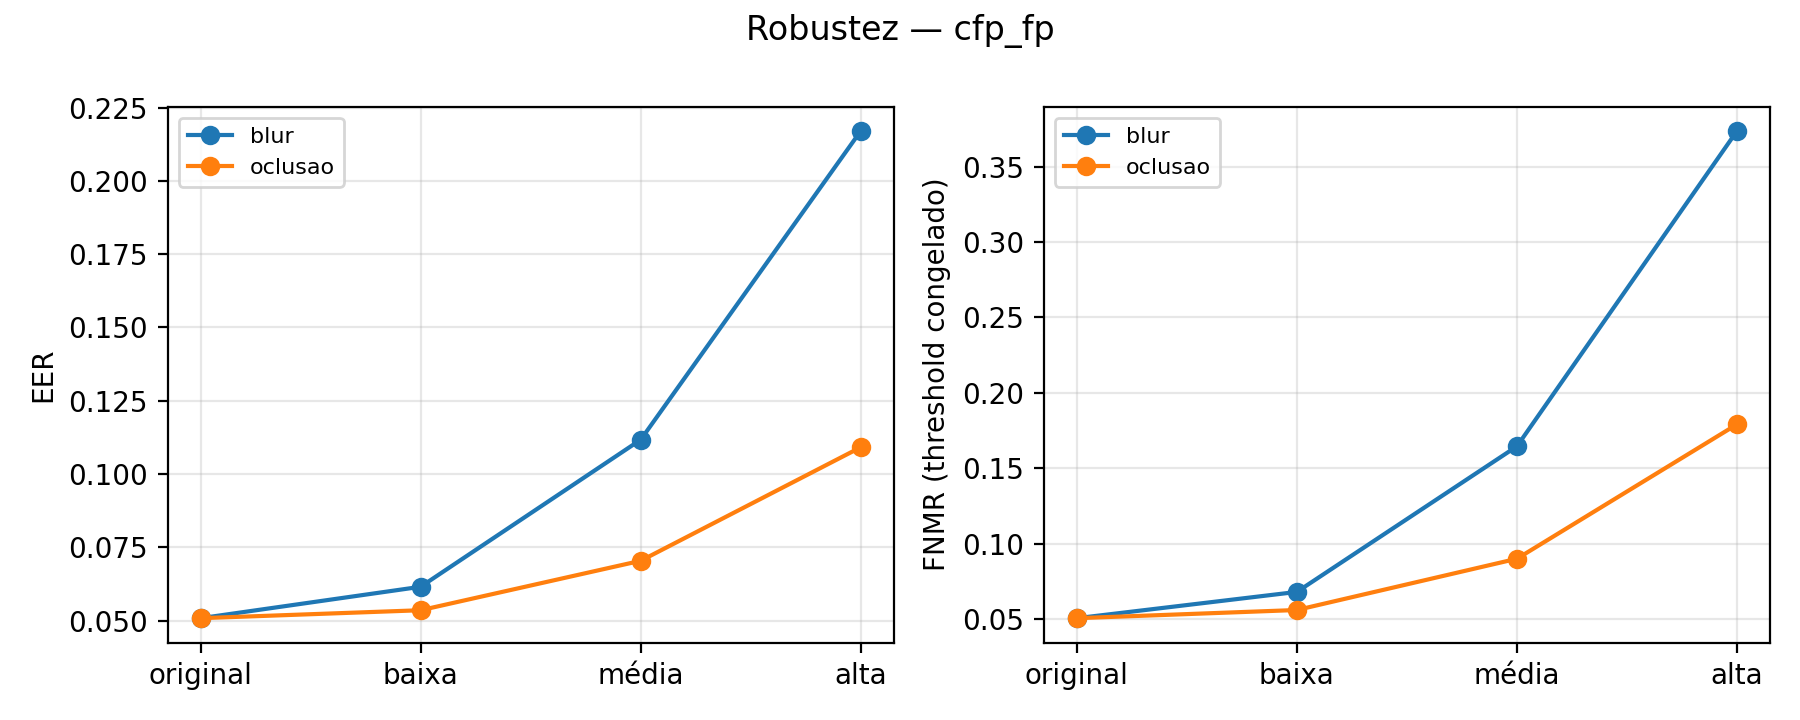
\includegraphics[width=\columnwidth]{robustness/robustness.png}
\caption{EER e FNMR (threshold congelado) sob desfoque e oclusão no CFP-FP.}
\label{fig:robustez}
\end{figure}
\todo{Discutir a curva: a partir de qual nível o desempenho cai; desfoque afeta também a
detecção (FTA); oclusão afeta só a CNN.}

\subsection{Alinhamento}
\todo{O alinhamento piora as duas bases (CFP-FP: EER \eerAlnCFP\% vs.\ \eerCFP\%;
LFW: \eerAlnLFW\% vs.\ \eerLFW\%). Explicação: o modelo foi pré-treinado com recortes
pela bbox, com mais contexto (testa, queixo, cabelo); o template ArcFace gera um
recorte mais justo e com outra geometria, fora da distribuição de treino. Lição:
o pré-processamento deve seguir o do pré-treino.}

\subsection{Análise de erros}
\begin{figure}[t]
\centering
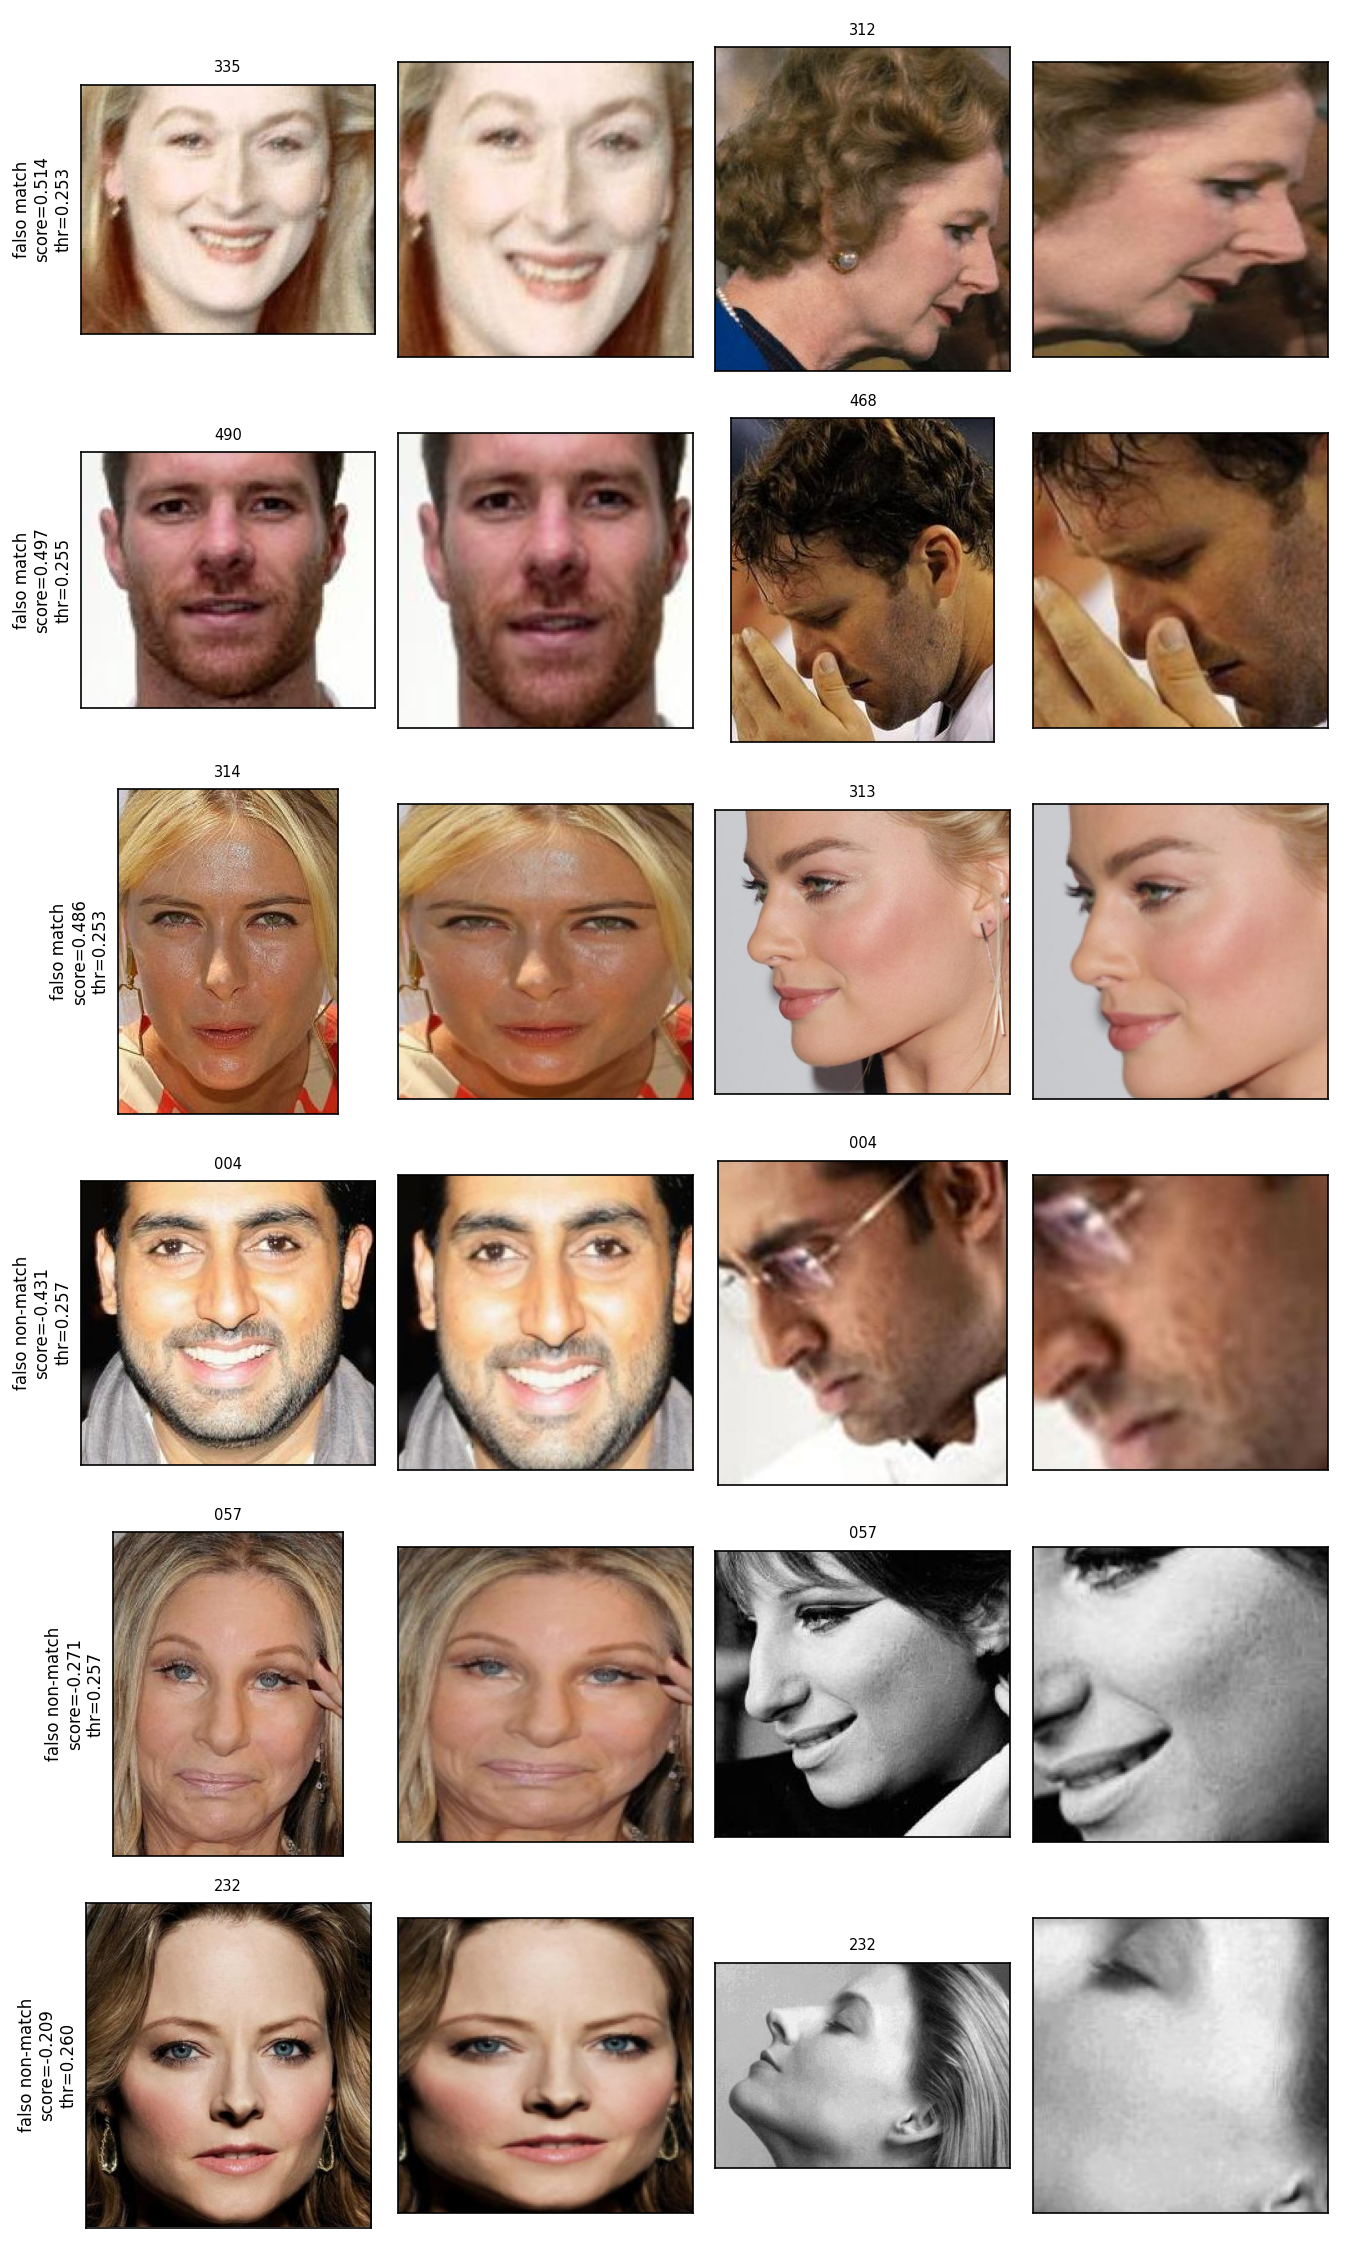
\includegraphics[width=\columnwidth]{cfp_fp_bbox/errors.png}
\caption{Três falsos matches (acima) e três falsos non-matches (abaixo) no CFP-FP.}
\label{fig:erros}
\end{figure}
\todo{Hipótese para cada caso (perfil extremo, oclusão, iluminação, semelhança entre
pessoas, detecção errada).}

\subsection{Comparação com a literatura}
\todo{Comparar com os números de referência (mesmo protocolo), destacando que os modelos
de ponta usam perdas de margem angular e bases de treino maiores.}

\subsection{Limitações}
O VGGFace2, o CFP e o LFW são compostos por celebridades, então pode haver identidades
em comum entre o pré-treino e o teste. O tempo medido não inclui a detecção. O modelo é
usado congelado, sem adaptação ao cenário de perfil. \todo{outras}

% =====================================================================
\section{Conclusão}
\todo{Síntese dos achados (3--4 frases com números) e perspectivas: fine-tuning em
perfis, perdas de margem angular, alinhamento sensível à pose.}

\bibliographystyle{IEEEtran}
\bibliography{refs}

\end{document}
